\documentclass[../main.tex]{subfiles}
\graphicspath{{\currfiledir}}
\begin{document}
\chapter{Terminology}
TODO intro?
\section{Grapheme}
\textcquote[204]{crystal2010}{Graphemes are the smallest units in a writing system capable of 
causing a contrast in meaning.}
In linguistics, graphemes are often placed in angle brackets, e.g. \grapheme{a} or \grapheme{b}.
Sometimes \emph{graphemes} are called \emph{signs}.
The term \emph{sign} and \emph{grapheme} are considered to be equivalent and 
interchangeable throughout this work.

\section{Graph and allograph}
\textcquote[204]{crystal2010}{Graphemes are abstract units which may adopt a variety of forms 
\elide Each of these possible forms is known as \emph{graphs}\elide
There is a vast amount of physical variation in the shapes of graphs that does not affect the 
underlying identity of the grapheme\elide 
When graphs are analyzed as variants of a grapheme, they are known as \emph{allographs}.}
The Maya script uses a lot of allographs.
For example, the syllable \syllable{u} can be written in many ways all having the same meaning.
See~\ref{fig:terminology-grapheme-u-allographs} for a selection of allographs.
\begin{center}
    
\includegraphics[width=\textwidth,keepaspectratio]{img/grapheme-u-allographs}
    \captionof{figure}{Some allographs of the grapheme \grapheme{u}}
    \label{fig:terminology-grapheme-u-allographs}
\end{center}

\section{Hieroglyph and glyph}
The term \emph{hieroglyph} and \emph{glyph} are not precise terms.
Both are used in epigraphic literature, to address a group of one or more graphemes.
\textcquote[1]{bricker1986}{A ``glyph'' is a sign that can occur alone or in combination with 
other signs}.
\textcquote[34]{knorozov1967}{A hieroglyph consists of several graphemes, which are joined 
in writing}. 
Both expressions are considered to be equivalent and interchangeable throughout this work.
\emph{Glyphs} can represent a syllable, a single word or even a whole phrase 
(\cite[23]{macrilooper2003}).

For example, the glyph~\ref{fig:terminology-glyphs-utzapaw} consists of the 
graphemes \grapheme{u}, \grapheme{tz\glottalstop{}a} and \grapheme{wa} representing the phrase
\mayan{u tz\glottalstop{}apaw}, ``she/he erects it''.
% LTeX: enabled=false
The glyph~\ref{fig:terminology-glyphs-ixwinikhaabajaw} consisting of the 
graphemes \grapheme{ix}, \grapheme{winikhaab} and \grapheme{ajaw}
and represents the noble title \mayan{ix winikhaab ajaw}, ``Ruler Lady Winikhaab''.
\begin{figure}
    \centering
    \subfloat[][]{
        \centering
        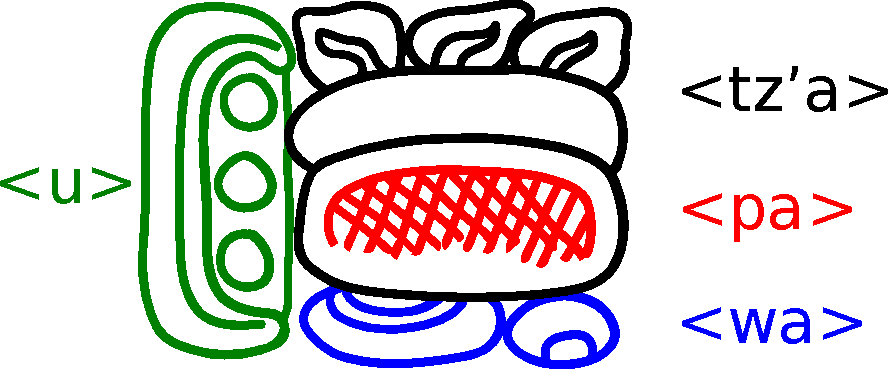
\includegraphics[height=\glyphblockheight]{img/glyphs-utzapaw}
        \label{fig:terminology-glyphs-utzapaw}
    }
    \subfloat[][]{
        \centering
        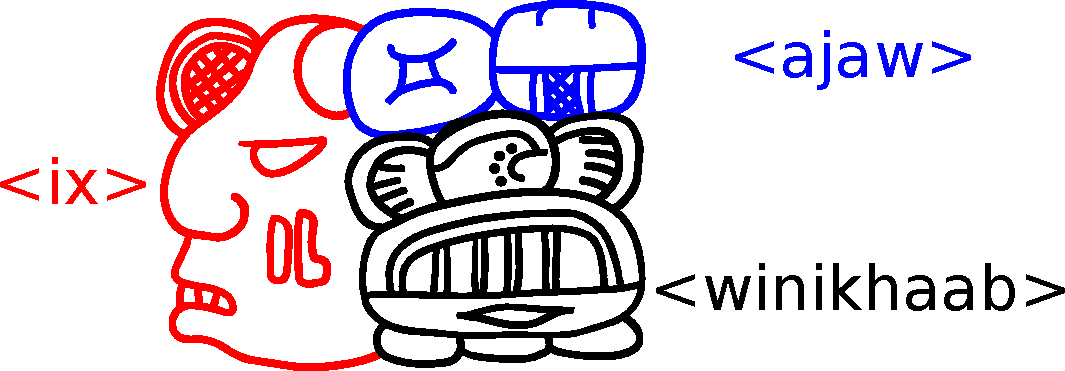
\includegraphics[height=\glyphblockheight]{img/glyphs-ixwinikhaabajaw}
        \label{fig:terminology-glyphs-ixwinikhaabajaw}
    }
    \caption[Sample glyphs]{Sample glyphs: graphemes are distinguished by different colors.\\
            \subref{fig:terminology-glyphs-utzapaw} \mayan{u tz\glottalstop{}apaw};
            \subref{fig:terminology-glyphs-ixwinikhaabajaw} \mayan{ix winikhaab ajaw} 
            (\authordrawings).}
\end{figure}
% LTeX: enabled=true

\section{Glyph block and collocation}
One or more \emph{Glyphs} are usually arranged in regular rectangular shapes called a 
\emph{glyph block}.
Sometimes they are also called \emph{collocation}.
\textcquote[1]{bricker1986}{A ``collocation'' is a group of signs that occupies a 
defined space, or block, in a hieroglyphic text.}
\textcquote[23]{macrilooper2003}{The rectangular shape of \emph{glyph blocks} results from 
the arrangement of texts into rows and columns}.
\todo{Image/drawing which shows rows and columns of glyphs}

\section{Theory in decipherment}
\textcquote[2]{zender2017}{The type of writing system must be known}.
As Johannes Friedrich already stated:
\blockquote[{\cite[152]{friedrich1957}}]{The decipherment of any unknown script or language 
presupposes the availability of some clue or reference; nothing can be deciphered out of nothing. 
In those cases where one has absolutely no possibility available to link the unknown to 
something known, \elide no real or lasting result can be accomplished}


\subsection{Script typology}
For successful decipherment process, it is crucial to know the fundamental structure of the signs.
The type of the script can either be alphabetic, syllabic, logographic or a combination of them.
In order to classify an unknown writing system, the number of signs employed in the scripts
can hint what type of writing system one deals with.
% LTeX: enabled=false
Johannes Friedrich observed:
\blockquote[{\cite[152]{friedrich1957}}]{\elide~the number of the written symbols usually warrants a 
conclusion as to whether the script is alphabetic, a pure syllabary (as in the Cypriote) or a
mixture of ideographic word-signs and syllabic signs (like the cuneiform writing or the Hittite
hieroglyphic script). A script consisting of less than thirty signs will presumably turn out to
be alphabetic\elide~Scripts containing fifty, a hundred or even several hundred different symbols
may justifiably be regarded beforehand as more or less complicated syllabic systems of writing,
perhaps employing also word-signs\elide}.
% LTeX: enabled=true
Based on Ignace Gelb (\cite[115]{gelb1963}), Michael Coe (\cite[43]{coe1992}) compiled a list
of writing systems and compared their type with the number of distinct signs
(see~\ref{table:terminology-writing-systems-comparison}).
\begin{table}[!ht]
    \centering
    \begin{tabular}{llc}
        \textbf{Type}                                                     & \textbf{Writing system} & \textbf{\# of signs} \\
        \multirow[t]{5}{20em}{\textbf{Logographic and Logosyllabic}\\
        Assigns a morpheme/word to each grapheme\\
        Logograms are either used for their semantic of syllabic values}  \\
                                                                          & Sumerian                & 600+ \\
                                                                          & Egyptian                & 2500 \\
                                                                          & Hittite Hieroglyphic    & 497 \\
                                                                          & Chinese                 & 5000+ \\        
        \\
        \multirow[t]{5}{20em}{\textbf{Syllabic}\\
        Assigns a syllable to each grapheme}                              \\
                                                                          & Persian                 & 40 \\
                                                                          & Linear B                & 87 \\
                                                                          & Cypriot                 & 56 \\
                                                                          & Cherokee                & 85 \\
        \\
        \multirow[t]{4}{20em}{\textbf{Abugida/Alphabetic Syllabary}\\ 
        Assigns a consonant to each grapheme\\
        Vowels or the absence of vowels are indicated by diacritics}      \\
                                                                          & Ethiopic                &  ca. 200 \\
                                                                          \\
                                                                          \\
        \\
        \multirow[t]{3}{20em}{\textbf{(Augmented) Abjad}\\
        Assigns a consonant to each grapheme\\
        In augmented abjad some voxels are added} \\
                                                                          & Phoenician              & 22 \\
                                                                          & Ugaritic                & 30 \\
        \\                                                                 
        \multirow[t]{8}{20em}{\textbf{(Augmented) Alphabet}\\
        Assigns a vowel or consonant to each grapheme}                    \\
                                                                          & English                 & 26 \\
                                                                          & Anglo-Saxon             & 31 \\
                                                                          & Sanskrit                & 35 \\
                                                                          & Etruscan                & 20 \\
                                                                          & Russian                 & 36 \\
                                                                          & Hebrew                  & 22 \\
                                                                          & Arabic                  & 28 \\
                                                                          & Coptic                  & 30 \\
    \end{tabular}
    \caption{Writing systems, their types and their number of distinct signs 
             (after~\cites[43]{coe1992}[730]{daniels1990}[88]{coulmas1991}{ritner1996})}
    \label{table:terminology-writing-systems-comparison}
\end{table}
So, in nutshell, to get a sense for the script type one can count the number of individual signs.
According to the table~\ref{table:terminology-writing-systems-comparison}, it should be possible
to narrow the number of possible script types.
The Maya text corpus is sufficiently big with 10,000 texts written on stone, wood, stucco, 
walls, pottery and four Post-Classic codices (\cite[151]{houstoncoe2003}).

\subsection{Corpus}
The database of texts (aka corpus) must be large enough so that sign catalogs can be created from it 
and analyzes of different text passages against each other allow effective comparisons 
(\cites[2]{zender2017}[44]{coe1992}).

\subsection{Language}
The language is crucial for any decipherment attempt.
If the languages died out or isn't spoken anymore, some ancestral or reconstructed 
version or some knowledge of the language family must be known (\cite[44]{coe1992}).
Marc Zender states \textcquote[3]{zender2017}{Absent some external evidence of the language, 
decipherment is impossible}.
However, Classic Maya --- the language of the Maya hieroglyphs ---  died out.
Although decipherment is challenging, it is possible to reconstruct texts by comparison 
with existing Maya languages as Christian Prager stated (\cite[6]{prager2018},my translation): 
\quotemytranslated[6]{prager2018}
% LTeX: enabled=false
{
    Es kann ausschließlich durch den Vergleich der 30 heute noch 
    gesprochenen Mayasprachen rekonstruiert werden. 
    Darüber hinaus ist vieles vom kulturellen Vokabular der vorspanischen Zeit als Folge der 
    Kolonisation verloren gegangen und bleibt bis heute eine große Herausforderung bei der 
    weiteren Entzifferung der Mayaschrift.
}
% LTeX: enabled=true
{
    It [Classic Maya] can only be reconstructed by comparing the 30 Mayan languages still 
    spoken today. 
    In addition, much of the cultural vocabulary of the pre-Hispanic period was lost as a result of 
    colonization and remains a major challenge in further decipherment of Maya writing 
    to this day.
}

\subsection{Cultural context}
\textcquote[44]{coe1992}{The cultural context of the script should be known, above all 
traditions and histories giving place-names, royal names and titles, and so forth.}
Well known place names, royal names or titles which occur in unknown script
play an important role in decipherment as they might hint how the fundamental mechanics of 
the writing system work.
One great example how royal names of titles helped to create an important insight of an unknown 
script, was the breakthrough Jean-Fran\c{c}ois Champollion had in deciphering the 
Egyptian hieroglyphs when analyzing the so-called Rosetta Stone which had a text written in 
three different writing systems, namely Greek, Demotic and Egyptian hieroglyphs.
Jean-Fran\c{c}ois Champollion focused on names of rulers which have been written both in 
Greek and in Egyptian hieroglyphs. 
Since Greek was well understood, the bilingual script helped him to compare the Greek writing with 
the Egyptian hieroglyphs.
Jean-Fran\c{c}ois Champollion realized, that in Egyptian hieroglyphs the names of personages 
are written in cartouches (\cite[215]{coulmas1991}).
One of the Greek names on the Rosetta Stone was \emph{Ptolemy}.
When comparing the name with hieroglyphs framed in cartouches, he deduced the phonetic writing 
of Ptolemy in Egyptian hieroglyphs (see~\ref{fig:terminology-ptolemy-cartouche}).
This insight opened the possibility to assign phonetic values to hieroglyphic signs and 
played a major role to decipher Egyptian hieroglyphs. 
\begin{center}
    
\includegraphics[width=.7\textwidth,keepaspectratio]{img/ptolemy-cartouche}
    \captionof{figure}{Ptolemy written in Egyptian hieroglyphs (read from right to left) with 
                       phonetic decipherment (\authordrawings)}
    \label{fig:terminology-ptolemy-cartouche}
\end{center}

% LTeX: enabled=false

In the 1960s David Kelley was able to show that a sequence of signs actually represent the name
of a Maya ruler (\cite{kelley1962a}).
He could show that with the help of Landa's abecedary 
(see \ref{fig:terminology-landa-relacion-folio-45r}) several sign sequences in the temples of
Chich\'{e}n Itz\'{a} denote the name of the ruler \mayan{K\glottalstop{}ak\glottalstop{}upakal}.
By cross-referencing this name with the book of Chilam Balam of Chumanyel --- a colonial source
written in Yucatec Maya with Latin letters he could identify that these inscription indeed
mention the name of the Maya ruler (\cite{kelley1968}).

Tu uucpiz tun Uaxac Ahau u katunil, laix u katunil cimci Chakanputin tumen Kak-u-pacal yetel Tec Uilue.
In the seventh tun of Katun 8 Ahau, this was the katun when Chakanputun perished at the hands of Kak-u-pacal and Tec Uilu

\cite[51,141]{roys1933}
% LTeX: enabled=true

% LTeX: enabled=false
\begin{figure}
    \centering
    \subfloat[][]{
        \centering
        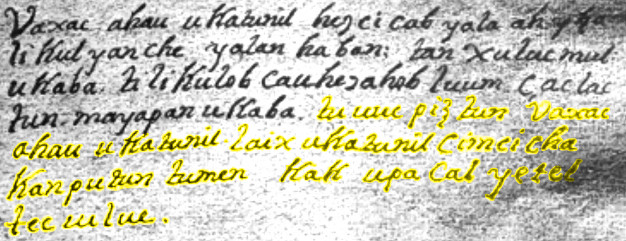
\includegraphics[width=0.63\textwidth]{img/chilam-balam-kakupakal}
        \label{fig:terminology-chilam-balam-kakupakal}
    }
    \subfloat[][]{
        \centering
        
\includegraphics[width=0.32\textwidth]{img/chichen-itza-monjas-lintel-2-kakupakal}
        \label{fig:terminology-chichen-itza-monjas-lintel-2-kakupakal}
    }
    \caption[K\glottalstop{}ak\glottalstop{}upakal in the colonial sources and inscriptions]
             {The name \mayan{K\glottalstop{}ak\glottalstop{}upakal} in the colonial sources and 
             in the inscriptions of Chich\'{e}n Itz\'{a}.
             \subref{fig:terminology-chilam-balam-kakupakal} page 51 from the book of 
             Chilam Balam of Chumayel.
             \subref{fig:terminology-chichen-itza-monjas-lintel-2-kakupakal}
             Hieroglyphic writing from Chich\'{e}n Itz\'{a} Monjas Lintel 2 (B1) (\authordrawings).}
\end{figure}
% LTeX: enabled=true


TODO maya context
rulers, place names, Colonial sources
Kakupakal
    - David H. Kelley - Glyphic Evidence for a Dynastic Sequenced Quirigua
    - David H. Kelley - Kakupakal and the Itzas

\subsection{Bilingual, biscript, or similar constraint}
Any clue as to what the content of the text might be is very important in deciphering an 
unknown script.
Bilingual scripts combining the unknown script with a well-known writing system helps to
verify the decipherment efforts (\cite[44]{coe1992}).
It can also be used to cross-reference readings of places, personage, titles etc. 
\textcquote[151]{houstoncoe2003}{If the script is logo-syllabic or heavily logographic, 
there should be accompanying pictorial references \elide to apply to the texts}.

Diego de Landa, a bishop who lived in Yucat\'{a}n in the 16th century, recorded aspects
of Maya writing in his work Relaci\'{o}n de las cosas de Yucat\'{a}n 
Even though his authorship is questionable (\cite{restallchuchiak2002}), this manuscript contains 
many aspects of Maya writing.
It contains vital information about the Maya calendars, the Maya signs for day names and month names
together with Spanish transcriptions.
It also contains the so-called ``Landa alphabet'' which basically represents a 
partial syllabary assigning a set of signs a phonetic value 
(\ref{fig:terminology-landa-relacion-folio-45r}).
Additionally, the manuscript includes two sentences both written in Maya hieroglyphs and 
Latin letters.
\begin{center}
    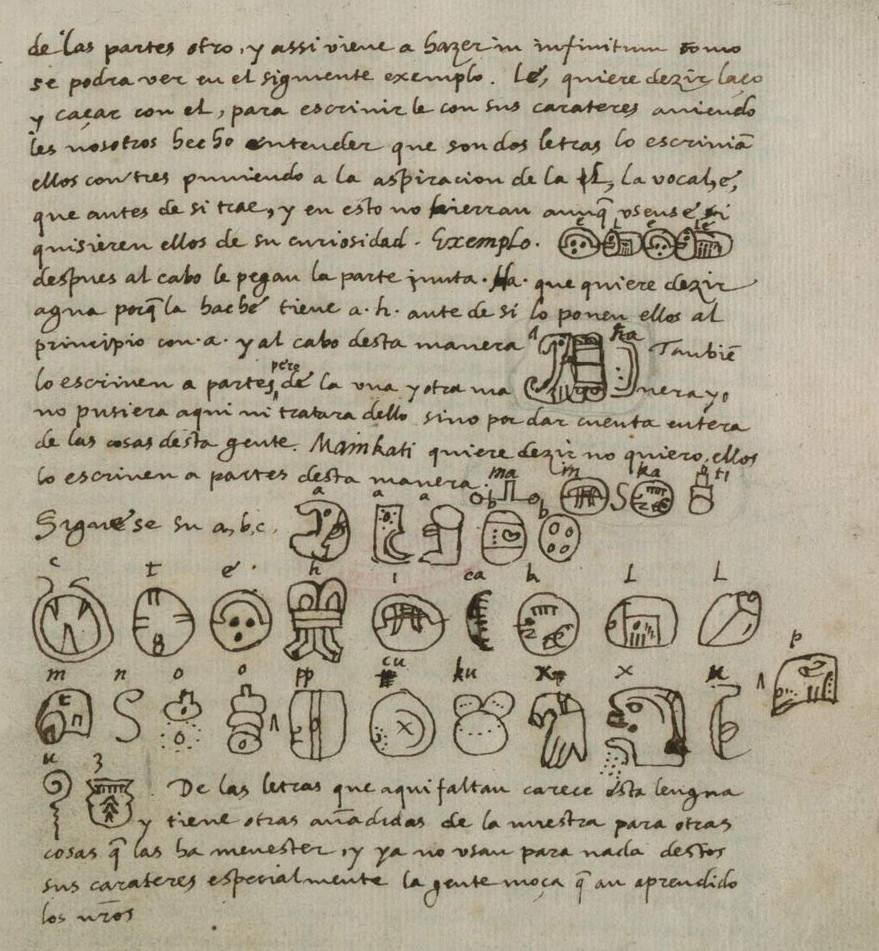
\includegraphics[width=0.8\textwidth,keepaspectratio]{img/landa-relacion-folio-45r}
    \captionof{figure}{Page 45r from Diego de Landa's manuscript containing the Landa alphabet 
                       (Courtesy of the Real Academia de la Historia~\cite{landa1567})}
    \label{fig:terminology-landa-relacion-folio-45r}
\end{center}
Besides this bilingual resource, many Maya writings combine text with imagery.
\textcquote[152]{houstoncoe2003}{Realistic, narrative pictures accompany most texts, usually 
illustrating the actions of the people or gods talked about in the writing.}

\section{Cataloging of signs}
One of the first steps to analyze an unknown writing system, is to identify distinctive graphemes 
and their allographs. 
In the past, several sign catalogs have been proposed.
Yuri Knorozov created a sign catalog in his work (\cite[109\psq]{knorozov1967}).
William E. Gates' and G\"unter Zimmermann's catalogs (\cite{gates1931},~\cite{zimmermann1956}) are 
based on the Maya codices but did not include the signs from the inscriptions 
(\cite[4]{thompson1962catalog}). 
Eric Thompson extended G\"unter Zimmermann's idea and categorized all signs into affixes, main signs 
(including animal heads) and portrait signs (\cite[4]{thompson1962catalog}).
His catalog covers the Maya codices, the monumental inscriptions and other writings 
(e.g.\ ceramics, vessels, bones).
All catalogs assigned a number to each sign/grapheme.
To distinguish between the different catalog systems, it is common to use a prefix in 
conjunction with the number.
So, for example, all Thompson numbers are labeled with the prefix ``T'', e.g. \thompson{510}.

In 2003, Martha J. Macri and Matthew G. Looper proposed a new system which assigns all graphemes
a code consisting of three digits (\cite[21,25]{macrilooper2003}).
The first two digits specifies the category of the sign 
(e.g. A for animals, M for signs with hands etc.) whereas the third digit is an arbitrary number
sequencing the different graphemes.

The project ``Text Database and Dictionary of Classic Mayan'' (abbr. TWKM) (\cite{twkm2014}) lead by 
Prof.\ Dr.\ Nikolai Grube of the Department of Anthropology of the Americas at the University of 
Bonn is currently compiling an updated and revisited version of Thompson's sign catalog.
% LTeX: enabled=false
Christian Prager states, \textcquote{prager2020}{we are currently evaluating and revising Eric 
Thompson’s Catalog of Maya Hieroglyphs (1962). 
We are critically scrutinizing his system with the help of his original grey cards and 
supplementing it with signs that were not included in Thompson’s original catalogue. 
Despite its known shortcomings and incompleteness, his catalogue is still regarded as the 
standard work for Maya epigraphers, which is why we adopt Thompson’s nomenclature while 
removing misclassifications and duplicates, merging graph variants under a common nomenclature, 
and adding new signs or allographs to the sign index in sequence, starting with the number 1500.}
% LTeX: enabled=true

\subsection{Problems and limitations}
Having all these sign catalogs are a huge help to systematically analyze any writing system.
It is especially important when the writing system cannot be read.
As one could see above, researchers assign codes or numbers to address individual or 
even groups of signs.
Therefore, identifying graphemes are crucial to systematically build up a sign catalog.
Yet, determine them in an unknown writing system is challenging.
One way to approach this, is by segmenting the texts into distinct \emph{graphs}.
Researchers hereby followed the assumption that graphemes of a script are considered the same if 
they resemble each other in more features than either resembles any other.
\textcquote[34]{knorozov1967}{Two [signs] are identical when they are both composed of the same 
graphic elements\elide, whose drawing and disposition is sufficiently similar to allow them to 
be identified}.
However, if there is no control in terms of linguistics and content, 
this approach can be problematic.
Three major issues can occur when segmenting signs from an unknown writing system.
\begin{itemize}
    \item Allographs are interpreted as separate graphemes.
    \item Graphemes with distinct phonetic value and meanings are interpreted as allographs.
    \item Complex graphemes are split into its sub-graphemic components.
\end{itemize}
Especially in writing systems with many allographs like the Maya hieroglyphs,
allographs are sometimes not recognized and, instead, are interpreted as separate graphemes. 
Sometimes, signs are considered to be allographs because of their similarities, 
but, as later progress in decipherment has shown, were actually distinct graphemes.
Eric Thompson (\cite[12\psq]{thompson1962catalog}) recognized the method of segmentation as 
a potential source of false conclusions.
David Kelley (\cite{kelley1962b}) was able to show in his review of Thompson's sign catalog that
some T-numbers represent more than one grapheme 
(e.g. \thompson{683a} and \thompson{T683b}~\ref{fig:terminology-t683a-t683b}) 
and some T-numbers are allographs of another 
(e.g. \thompson{589} and \thompson{T607}~\ref{fig:terminology-t589-t607}).
% LTeX: enabled=false
\begin{figure}
    \centering
    \subfloat[][]{
        \centering
        
\includegraphics[height=\glyphblockheight]{img/T683a-T683b}
        \label{fig:terminology-t683a-t683b}
    }
    \subfloat[][]{
        \centering
        
\includegraphics[height=\glyphblockheight]{img/T589-T607}
        \label{fig:terminology-t589-t607}
    }
    \caption[Questionable T-number assignment in Thompson's catalog]{Questionable T-number 
            assignment in Thompson's catalog (after Kelley).
            \subref{fig:terminology-t683a-t683b} \grapheme{winik} and \grapheme{ja} 
            assigned to \thompson{683};
            \subref{fig:terminology-t589-t607} \grapheme{ho} assigned to \thompson{589} and 
            \thompson{607} (\authordrawings).}
\end{figure}
% LTeX: enabled=true
Despite merging unrelated graphs or separating allographs which actually belong to each other,
the Maya writing system also utilizes graphemes which consist of two or more subgraphemic 
components.
Those complex graphemes might not be recognized and therefore only its components are registered
as graphemes.
One of those complex graphemes, is the grapheme \grapheme{pas} ``dawn'' 
(\ref{fig:terminology-glyphs-pas}) which is built from
grapheme \grapheme{chan} ``sky'' (\ref{fig:terminology-glyphs-chan}), 
grapheme \grapheme{k\glottalstop} ``k\glottalstop{}in'' (\ref{fig:terminology-glyphs-kin}) and
grapheme \grapheme{kab} ``earth'' (\ref{fig:terminology-glyphs-kab}).
It can be found, for example, on Tikal Temple IV, Lintel 2 A7.
All three components are graphemes themselves, but in combination they form the complex 
grapheme \grapheme{pas} with its own phonetic value and meaning.
This grapheme doesn't show up in Thompson's sign catalog.
Later revisions and new catalogs like Macri and Looper (\cite{macrilooper2003}) added it as
separate grapheme and assigned it the code ZX2.
% LTeX: enabled=false
\begin{figure}
    \centering
    \subfloat[][]{
        \centering
        
\includegraphics[height=\glyphblockheight]{img/grapheme-PAS}
        \label{fig:terminology-glyphs-pas}
    }
    \subfloat[][]{
        \centering
        
\includegraphics[height=\glyphblockheight]{img/grapheme-CHAN}
        \label{fig:terminology-glyphs-chan}
    }
    \subfloat[][]{
        \centering
        
\includegraphics[height=\glyphblockheight]{img/grapheme-KIN}
        \label{fig:terminology-glyphs-kin}
    }
    \subfloat[]{
        \centering
        
\includegraphics[height=\glyphblockheight]{img/grapheme-KAB}
        \label{fig:terminology-glyphs-kab}
    }
    \caption[Grapheme \grapheme{pas}]{Grapheme \grapheme{pas}. Even though it consists of three 
             other graphemes, it represents a self-contained grapheme with separate phonetic and 
             meaning (\cite[139]{prager2018}).
             \subref{fig:terminology-glyphs-pas} \grapheme{pas} ``dawn'';
             \subref{fig:terminology-glyphs-chan} \grapheme{chan} ``sky'';
             \subref{fig:terminology-glyphs-kin} \grapheme{k\glottalstop{}in} ``sun'';
             \subref{fig:terminology-glyphs-kab} \grapheme{kab} ``earth'' (\authordrawings).}
\end{figure}
% LTeX: enabled=true

\end{document}
